\documentclass{exam}

\usepackage{units} 
\usepackage{graphicx}
\usepackage[fleqn]{amsmath}
\usepackage{cancel}
\usepackage{float}
\usepackage{mdwlist}
\usepackage{booktabs}
\usepackage{cancel}
\usepackage{polynom}
\usepackage{caption}
\usepackage{fullpage}
\usepackage{comment}
\usepackage{enumerate}
\usepackage{xfrac}

\newcommand{\degree}{\ensuremath{^\circ}} 
\everymath{\displaystyle}

% \begin{figure}[H]
%   \centering
%   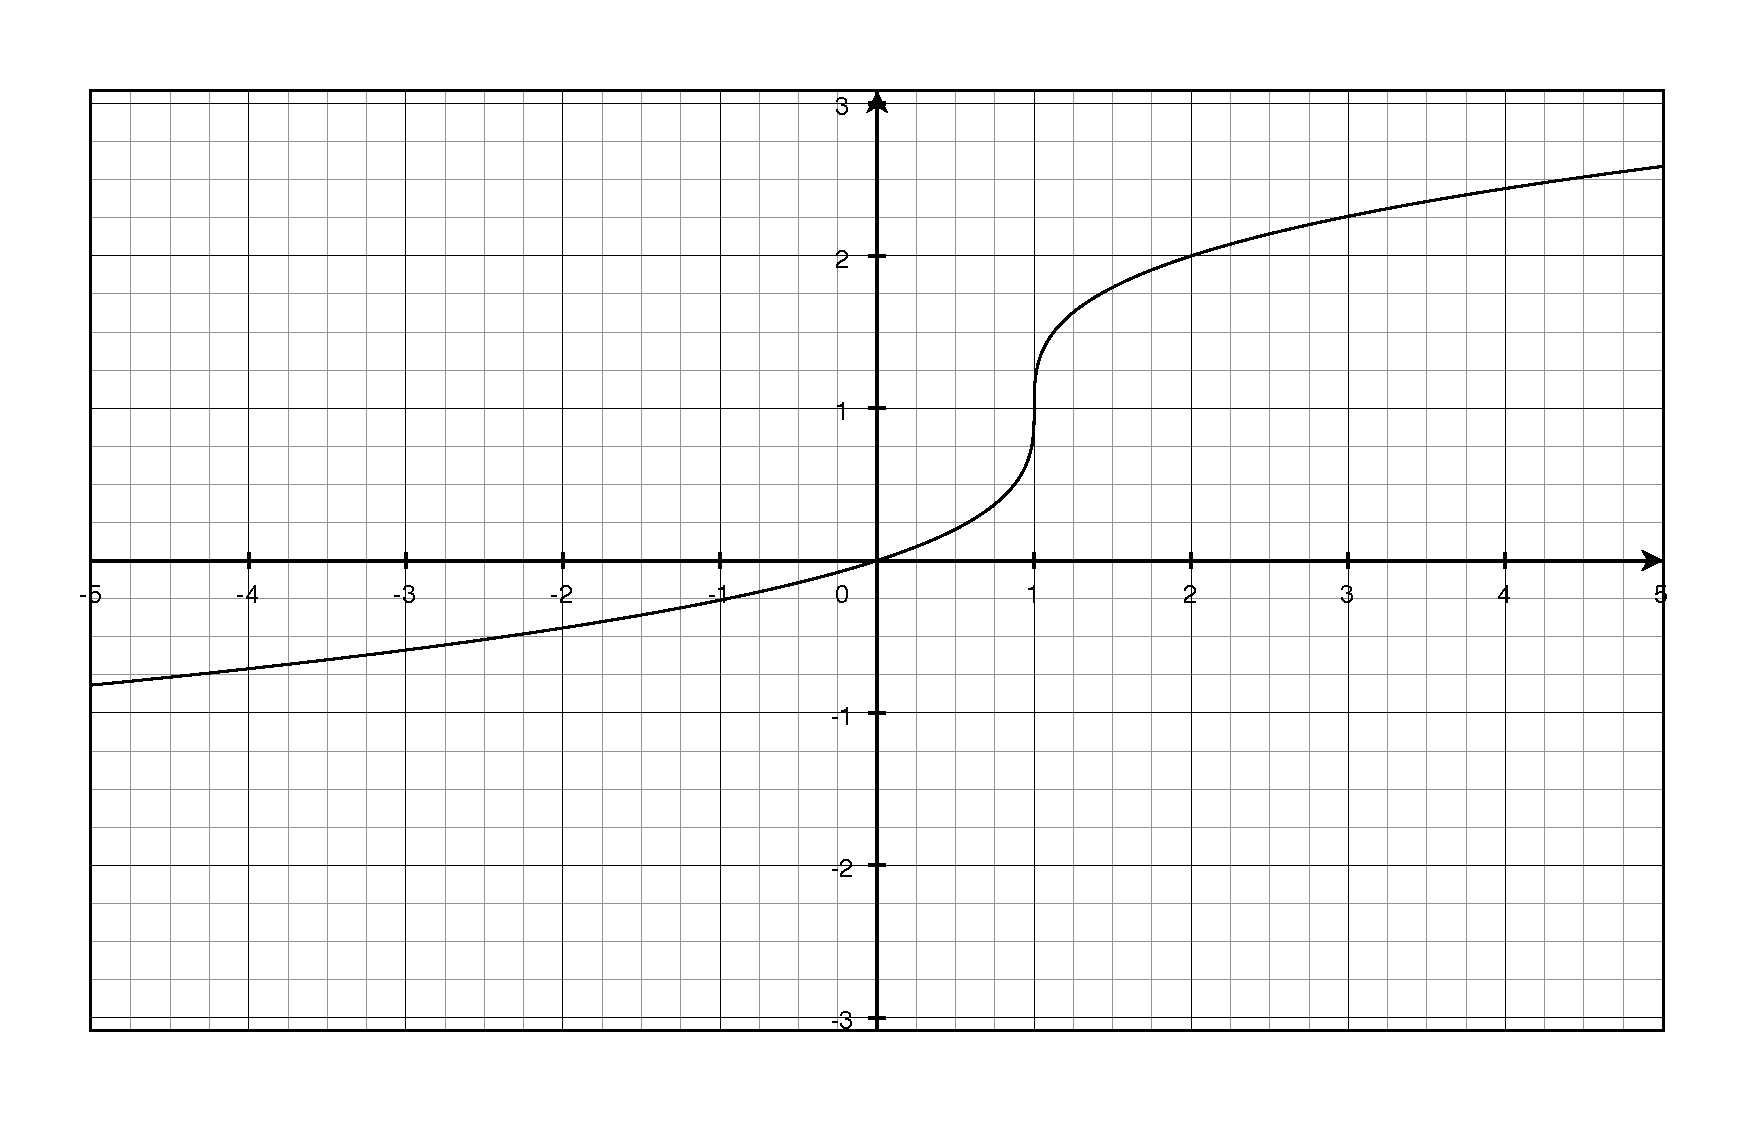
\includegraphics[scale=.3]{question7.eps}
%   \caption*{question 7}
% \end{figure}

% \begin{tabular}{cc}
%   \toprule
%   period & amplitude \\
%     $\pi$ & $2$ \\
%   \bottomrule
% \end{tabular}

\printanswers
\excludecomment{comment}

\ifprintanswers 
  \usepackage{2in1, lscape} 
\fi

\author{}
\date{\today}
\title{Math 142 \\ Homework Six}

\begin{document}

  \maketitle

  \section{Homework}
  Section 6.1: 

  \section{Extra Credit}
  Section 6.1: 76 and 84

  \ifprintanswers

    \begin{description}
      \item[76]
        There are four different quarter circles the cow can graze in:
        \begin{align*}
          A_1 &= \frac{1}{4} \pi \times 100^2 \approx \unit[3927 \pi]{ft^2} \\
          A_2 &= \frac{1}{4} \pi \times 50^2 \approx \unit[982]{ft^2} \\
          A_3 &= \frac{1}{4} \pi \times 30^2 \approx \unit[353]{ft^2} \\
          A_4 &= \frac{1}{4} \pi \times 40^2 \approx \unit[628]{ft^2} \\
        \end{align*}

        The total is:
        \[
          \unit[3927 \pi]{ft^2} + \unit[982]{ft^2} + \unit[353]{ft^2} + \unit[628]{ft^2} = \boxed{ \unit[5890]{ft^2} }
        \]
        
      \item[84]
        \begin{enumerate}[(a)]

          \item 
            Find the angular speed of the pedal sprocket
            \[
              \omega_{pedal} = 2 \pi \times 40 = \unit[80 \pi]{rad/m}
            \]

            Since the circumference of the wheel sprocket is half the circumference of the pedal sprocket, it turns
            twice for every turn of the pedal and its angular velocity is:
            Find the angular speed of the wheel sprocket:
            \[
              \omega_{wheel} = 2 \times \omega_{pedal} = \boxed{ \unit[160 \pi]{rad/m} } 
            \]

          \item 
            \[
              v_{bike} = 160 \pi \times 13 \approx \unit[ 6535 ]{in/m}
            \]

            Convert to mph which is a more usual unit for bike speed:
            \[
              \unit[ 6535 ]{in/m} \times \frac{\unit[1]{ft}}{\unit[12]{in}} \times \frac{\unit[1]{mi}}{\unit[5280]{ft}}
              \times \frac{\unit[60]{m}}{\unit[1]{hr}} \approx \boxed{ \unit[6.2]{mph} }
            \]


        \end{enumerate}
    \end{description}

    \section{Section 6.1}
    \begin{description}
      \item[1] 
        \[
          72 \degree \cdot \frac{2 \pi}{360 \degree} = \boxed{ \frac{2 \pi}{5} }
        \]

      \item[2] 
        \[
          54 \degree \cdot \frac{2 \pi}{360 \degree} = \boxed{ \frac{3 \pi}{10} }
        \]

      \item[3] 
        \[
          -45 \degree \cdot \frac{2 \pi}{360 \degree} = \boxed{ -\frac{\pi}{4} }
        \]

      \item[4] 
        \[
          -60 \degree \cdot \frac{2 \pi}{360 \degree} = \boxed{ -\frac{\pi}{3} }
        \]

      \item[5] 
        \[
          -75 \degree \cdot \frac{2 \pi}{360 \degree} = \boxed{ -\frac{5 \pi}{12} }
        \]

      \item[13] 
        \[
          \frac{7 \pi}{6} \cdot \frac{360 \degree}{2 \pi} = \boxed{ 210 \degree }
        \]

      \item[14] 
        \[
          \frac{11 \pi}{3} \cdot \frac{360 \degree}{2 \pi} = \boxed{ 660 \degree }
        \]

      \item[15] 
        \[
          - \frac{5 \pi}{4} \cdot \frac{360 \degree}{2 \pi} = \boxed{ -225 \degree }
        \]

      \item[16] 
        \[
          - \frac{3 \pi}{2} \cdot \frac{360 \degree}{2 \pi} = \boxed{ -270 \degree }
        \]

      \item[17] 
        \[
          3 \cdot \frac{360 \degree}{2 \pi} \approx \boxed{ 172 \degree }
        \]

      \item[25] 
        \begin{align*}
          50 \degree + 360 \degree & = \boxed{ 410 \degree } \\
          50 \degree + 720 \degree & = \boxed{ 770 \degree } \\
          50 \degree - 360 \degree & = \boxed{ -310 \degree } \\
          50 \degree - 720 \degree & = \boxed{ -670 \degree } \\
        \end{align*}

      \item[26] 
        \begin{align*}
          135 \degree + 360 \degree & = \boxed{ 495 \degree } \\
          135 \degree + 720 \degree & = \boxed{ 855 \degree } \\
          135 \degree - 360 \degree & = \boxed{ -225 \degree } \\
          135 \degree - 720 \degree & = \boxed{ -585 \degree } \\
        \end{align*}

      \item[27] 
        \begin{align*}
          \frac{3 \pi}{4} + 2 \pi & = \boxed{ \frac{11 \pi}{4} } \\
          \frac{3 \pi}{4} + 4 \pi & = \boxed{ \frac{19 \pi}{4} } \\
          \frac{3 \pi}{4} - 2 \pi & = \boxed{ - \frac{5 \pi}{4} } \\
          \frac{3 \pi}{4} - 4 \pi & = \boxed{ - \frac{13 \pi}{4} } \\
        \end{align*}

      \item[28] 
        \begin{align*}
          \frac{11 \pi}{4} + 2 \pi & = \boxed{ \frac{19 \pi}{4} } \\
          \frac{11 \pi}{4} + 4 \pi & = \boxed{ \frac{27 \pi}{4} } \\
          \frac{11 \pi}{4} - 4 \pi & = \boxed{ - \frac{5 \pi}{4} } \\
          \frac{11 \pi}{4} - 6 \pi & = \boxed{ - \frac{13 \pi}{4} } \\
        \end{align*}

      \item[31] $430 \degree = 70 \degree + 360 \degree$
        The angles are \fbox{ coterminal }.

      \item[32] $330 \degree = 360 \degree - 30 \degree$
        The angles are \fbox{ coterminal }.

      \item[33] $\frac{17 \pi}{6} = \frac{5 \pi}{6} + 2 \pi$
        The angles are \fbox{ coterminal }.

      \item[34] The angles are \fbox{ not coterminal }.

      \item[35] $875 \degree = 155 \degree + 720 \degree$
        The angles are \fbox{ coterminal }.

      \item[36] The angles are \fbox{ not coterminal }.

      \item[37] $733 \degree - 720 \degree = \boxed{ 13 \degree }$

      \item[38] $361 \degree - 360 \degree = \boxed{ 1 \degree }$

      \item[39] $1110 \degree - 1080 \degree = \boxed{ 30 \degree }$

      \item[40] $-100 \degree + 360 \degree = \boxed{ 260 \degree }$

      \item[41] $-800 \degree + 1080 \degree = \boxed{ 280 \degree }$

      \item[42] $1270 \degree - 1080 \degree = \boxed{ 190 \degree }$

      \item[43] $\frac{17 \pi}{6} - 2 \pi = \boxed{ \frac{5 \pi}{6} }$

      \item[44] $- \frac{7 \pi}{3} + 4 \pi = \boxed{ \frac{5 \pi}{3} }$

      \item[45] $87 \pi - 86 \pi = \boxed{ \pi }$

      \item[46] $10 - 2 \pi \approx \boxed{ 3.7168 }$

      \item[47] $\frac{17 \pi}{4} - 4 \pi = \boxed{ \frac{\pi}{4} }$

      \item[48] $\frac{51 \pi}{2} - 25 \pi = \boxed{ \frac{\pi}{2} }$

      \item[49]
        Find the angle in radians:
        \[
          (360 \degree - 140 \degree) \times \frac{2 \pi}{360 \degree} = \frac{11 \pi}{9}
        \]

        The arc length is:
        \[
          \frac{11 \pi}{9} \times 5 = \frac{55 \pi}{9} \approx \boxed{ 19.2 }
        \]

      \item[50]
        \begin{align*}
          5 \alpha & = 10 \\
          \alpha   & = \boxed{ 2 } \\
        \end{align*}

      \item[51]
        \begin{align*}
          2 r & = 8 \\
          r   & = \boxed{ 4 } \\
        \end{align*}

      \item[52]
        Find the angle in radians:
        \[
          45 \degree \times \frac{2 \pi}{360 \degree} = \frac{\pi}{4}
        \]

        The arc length is:
        \[
          \frac{\pi}{4} \times \unit[10]{m} = \unit[ \frac{5 \pi}{2} ]{m} \approx \boxed{ \unit[7.85]{m} }
        \]

      \item[53]
        \[
          2 \times \unit[2]{m} = \boxed{ \unit[4]{m} } 
        \]

      \item[54]
        \begin{align*}
          5 \theta & = 6 \\
          \theta   & = \boxed{ \frac{6}{5} } \\
                   & \approx \boxed{ 68.7 \degree } \\
        \end{align*}

      \item[59]
        \begin{enumerate}[(a)]
          \item 
            Find the angle in radians:
            \[
              80 \degree \times \frac{2 \pi}{360 \degree} = \frac{4 \pi}{9}
            \]

            Find the area:
            \[
              A = \frac{1}{2} \times 8^2 \times \frac{4 \pi}{9} = \frac{128 \pi}{9} \approx \boxed{ 44.68 }
            \]

          \item
            \[
              A = \frac{1}{2} \times 10^2 \times 0.5 = \boxed{ 25 }
            \]
        \end{enumerate}

      \item[60]
        \begin{enumerate}[(a)]
          \item
            \begin{align*}
              12 & = \frac{1}{2} r^2 \times 0.7 \\
              r  & \approx \boxed{ 5.9 } \\
            \end{align*}

          \item 
            Find the angle in radians:
            \[
              150 \degree \times \frac{2 \pi}{360 \degree} = \frac{5 \pi}{6}
            \]

            Find the radius:
            \begin{align*}
              12 & = \frac{1}{2} r^2 \times \frac{5 \pi}{6} \\
              r  & \approx \boxed{ 3.0 } \\
            \end{align*}

        \end{enumerate}

      \item[61]
        \begin{align*}
          A & = \frac{1}{2} 10^2 \times 1 \\
            & = \boxed{ 50 } \\
        \end{align*}

      \item[62]
        Find the angle in radians:
        \[
          60 \degree \times \frac{2 \pi}{360 \degree} = \frac{\pi}{3}
        \]

        Find the area:
        \begin{align*}
          A & = \frac{1}{2} 3^2 \times \frac{\pi}{3} \\
            & = \boxed{ \frac{3 \pi}{2} } \\
        \end{align*}

      \item[67]
        The circumference of the tire is: $28 \pi$.  In 10,000 revolutions, the
        car travels 10,000 times the circumference or:
        \[
          10,000 \times 28 \pi \approx \unit[ 879,650 ]{in}
        \]

        Convert to miles:
        \[
          \unit[ 879,650 ]{in} \times \frac{ \unit[1]{ft} }{ \unit[12]{in}} \times \frac{ \unit[1]{mi} }{ \unit[5280]{ft} } \approx \boxed{ \unit[13.9]{mi} }
        \]

      \item[68]
        Convert 1 mile to inches:
        \[
          \unit[ 1 ]{mi} \times \frac{ \unit[5280]{ft} }{ \unit[1]{mi}} \times \frac{ \unit[12]{in} }{ \unit[1]{ft} } = \unit[63,360]{in}
        \]

        The circumference of the tire is: $30 \pi$.  Traveling $30 \pi$ inches per revolution, the number of revolutions required is:
        \[
          \unit[63,360]{in} \times \frac{\unit[1]{rev}}{\unit[30 \pi]{in}} \approx \boxed{ \unit[672]{revolutions} }
        \]

      \item[69]
        The angle between the two cities is: 
        \[
          40.5 \degree - 25.5 \degree = 15 \degree = \unit[ \frac{\pi}{12} ]{rad}
        \]

        The distance is:
        \[
          \unit[ \frac{\pi}{12} ]{rad} \times \unit[3960]{mi} \approx \boxed{ \unit[ 1037 ]{mi} }
        \]

      \item[71]
        In one day, the earth travels $\sfrac{1}{365}$ of it's orbit.  In radians, this is:
        \[
          \frac{1}{365} \times 2 \pi = \frac{2 \pi}{365}
        \]

        The arc length for this angle is:
        \[
          \frac{2 \pi}{365} \times \unit[ 93 \times 10^6 ]{mi} \approx \boxed{ \unit[1.6 \times 10^6]{miles} }
        \]

      \item[72]
        Convert to radians:
        \[
          7.2 \degree \approx \unit[0.12566]{rad}
        \]

        Find the radius:
        \begin{align*}
          0.12566 r & = 500 \\
          r         & \approx \boxed{ \unit[3979]{mi} } \\
        \end{align*}

      \item[73]
        Convert to radians:
        \[
          \frac{1}{60} \degree = \unit[ \frac{\pi}{10,800} ]{rad}
        \]

        Find the distance:
        \[
          \unit[ 3960 ]{mi} \times \frac{\pi}{10,800} \approx \boxed{ \unit[1.15]{mi} }
        \]

      \item[80]
        The time required for a rotation in hours is: 
        \[
          \unit[23]{hr} + \unit[ \frac{56}{60} ]{hr} + \unit[\frac{4}{3600}]{hr} \approx \unit[23.934]{hr}
        \]

        The angular velocity is:
        \[
          \omega = 23.934 \times 2 \pi = \unit[150.4]{rad/hr}
        \]

        The linear velocity is:
        \[
          \unit[150.4]{rad/hr} \times \unit[3960]{mi} \approx \boxed{ \unit[ 595,000 ]{mi/hr} }
        \]

      \item[81]
        The angular velocity is:
        \[
          \omega = 600 \times 2 \pi = \unit[1200 \pi]{rad/hr}
        \]

        The linear velocity in inches per minute is:
        \[
          \unit[1200 \pi]{rad/hr} \times \unit[11]{in} \approx \unit[41,469]{in/min}
        \]

        Convert to mph:
        \[
          \unit[41,469]{in/min} \times \frac{\unit[1]{ft}}{\unit[12]{in}} \times \frac{\unit[1]{mi}}{\unit[5280]{ft}} \times \frac{\unit[60]{min}}{\unit[1]{hr}} 
          \approx \boxed{ \unit[39]{mph} }
        \]


    \end{description}

  \else
    \vspace{1 cm}
    \begin{quote}
      \begin{em}
        TO DO
      \end{em}
    \end{quote}
    \hspace{1 cm} --Shunryu Suzuki
  \fi

\end{document}

